
\subsubsection{Synthèse des méthodes de compression basée sur les $K^2$-trees }

Nous avons présenté dans les parties précédentes les différentes méthodes de compression existantes basées sur la représentation $k^2$-trees, et expliqué le principe de fonctionnement de chaqu'une d'elles. Nous allons par la suit comparer entre ces méthodes et résumer nos recherches.

Une présentation synthétique de notre étude est fournie dans le tableau \ref{K2-trees-table}. Chaque ligne du tableau représente une méthode, tandis que chaque colonne
représente un aspect susceptible d’être utilisé dans la méthode (type de graphe, type de compression, structure en sortie). Nous constatons que toutes les méthodes de cette classe sont des méthodes de compression sans perte qui supportent les graphes orientés et non orientés, cependant nous remarquons une variation dans l'aspect temporelle, certains méthodes sont destinées aux graphes statiques comme $k^2$-trees de base et $k^2$-trees1, tandis que d'autres sont appliquées aux graphes dynamiques comme $k^n$-trees et d$k^2$-trees. Certains méthodes se distinguent aussi par le type de graphe comme $k^2$-treaps qui s'applique aux graphes pondérés et Att$k^2$-trees qui accepte les graphes étiquetés, attribués et multiples. Nous observons aussi que toutes les méthodes donnent en sortie une représentation succincte. le tableau résume aussi les résultats de l'application des méthodes sur des graphes de test. Les figures \ref{eu2005-k2} et \ref{k2-taux} sont des représentations visuelles des ces résultats.\\

La figure \ref{eu2005-k2} représente les résultats obtenues par l'application des méthodes de compression basées sur les $k^2$-trees sur le graphe eu-2005 en tenant compte de l’ordre chronologique de leurs apparitions. Les résultats sont sous forme de nombre de bits par liens. Nous remarquons que la première méthode de base donne un résultat de compression de 5.2bpe, ce nombre a diminué avec l'apparition des améliorations et des nouvelles méthodes. Nous constatons alors une amélioration contenue de l'efficacité de ces méthodes de manière générale surtout avec les améliorations proposées par \citep{brisaboa2014compact} et Delta$k^2$-trees où le nombre de bits atteint approximativement 3.22 bits par liens.

 \begin{figure}[H]
		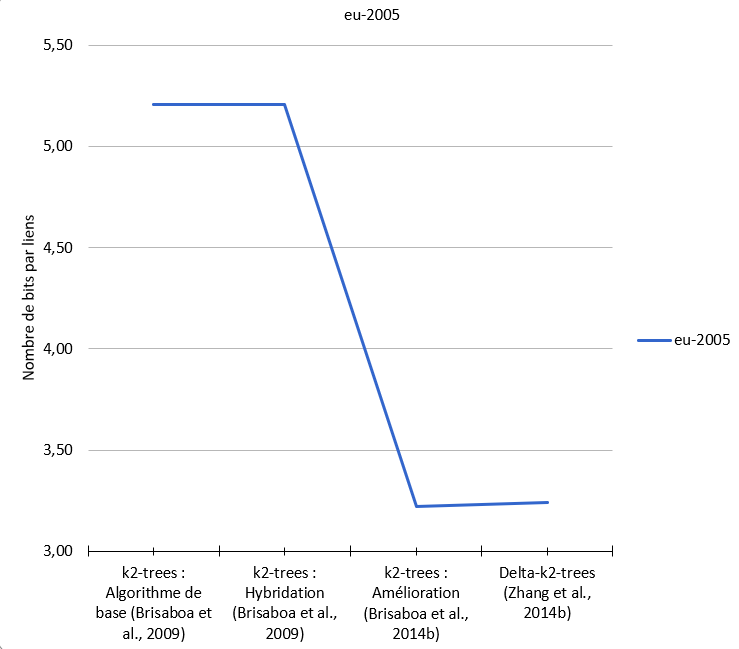
\includegraphics[height=10.5cm, width=16cm]{./ressources/image/eu2005-k2.png}
		\caption{Comparaison des performances des méthodes basées sur les $k^2$-trees appliquées sur le graphe eu2005 selon le nombre de bits par liens}
		\label{eu2005-k2}
	\end{figure}
	
A partir de la figure \ref{K2-trees-table} qui présente les résultats de l'application de différentes méthodes sur quatre graphes de test (CommNet, cond-mat, eu-2005, movilens10M) en fonction du taux de compression. Nous remarquons que entre $k^2$-trees et $k^2$-trees1, la méthode $k^2$-trees est nettement meilleure, cela s'explique par le fait que les graphes du web sont représentés par des matrices creuses et $k^2$-trees1 est mieux adaptée au matrices avec des zones de uns comme les matrices d'images par exemple.	Pour les graphes dynamiques, nous observons que $k^n$-trees donne de bons résultats par rapport à I$k^2$-trees mais avec une légère différence. Pour les graphes attribués, Att$k^2$-trees donne un très bon résultat avec un taux de compression de 93\%. 
	\begin{figure}[H]
		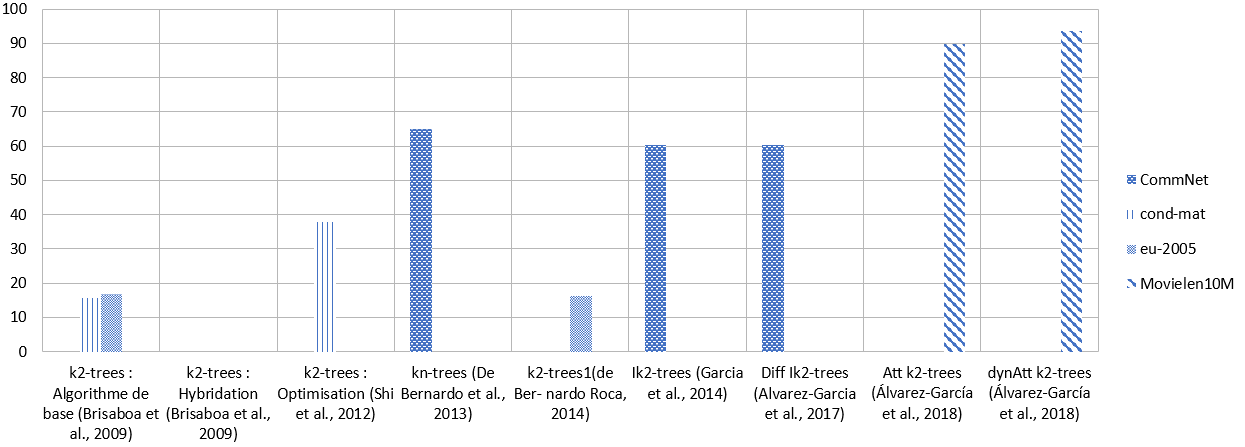
\includegraphics[height=9cm, width=18cm]{./ressources/image/k2-taux.png}
		\caption{Comparaison entre les méthodes basées sur les $k^2$-trees en fonction du taux de compression}
		\label{k2-taux}
	\end{figure}
	


    
 												
														\begin{landscape}
								\begin{table}
									\begin{tabular}{|C{3cm}|c|c|c|c|c|c|c|c|c|c|c|c|c|}
										\hline
										\multirow{2}{*}[-25pt]{     Article   }  & \multicolumn{5}{c|}{Graphe en entrée} & \multicolumn{2}{c|}{Compression} & \multicolumn{2}{c|}{Structure en sortie} & \multirow{2}{*}[-25pt]{Graphe de test} & \multirow{2}{*}[-25pt]{Résultat }  \\ \cline{2-10}
				     & \rotatebox[origin=c]{90}{ Orienté }  & \rotatebox[origin=c]{90}{ Non orienté } & \rotatebox[origin=c]{90}{ Statique } & \rotatebox[origin=c]{90}{ Dynamique } & \rotatebox[origin=c]{90}{ Autre Propriétés } &  \rotatebox[origin=c]{90}{ Avec perte } & \rotatebox[origin=c]{90}{ Sans perte } & \rotatebox[origin=c]{90}{ Succincte } & \rotatebox[origin=c]{90}{ Structurelle } & & \\ \hline				%%%%%%Fin du header
				
\hline  $k^2$-trees : Algorithme de base
   \citep{brisaboa2009k} 
   & \cmark & \cmark & \cmark & \xmark &  & \xmark &  \cmark & \cmark & \xmark	 & 		
	\begin{minipage}[t]{0.15\textwidth}
	eu-2005\\
	
	cond-mat
  \end{minipage}	
										 &
	\begin{minipage}[t]{0.4\textwidth}
	 5.21 bits/lien \\
	 taux de compression : 16.88\% \\
	 taux de compression : 15.58\% 
  \end{minipage}	\\

\hline $k^2$-trees : Hybridation \citep{brisaboa2009k} & \cmark & \cmark & \cmark & \xmark &  & \xmark &  \cmark & \cmark & \xmark  & 
										\begin{minipage}[t]{0.15\textwidth}
	eu-2005
  \end{minipage}	
										 &
	\begin{minipage}[t]{0.4\textwidth}
	 5.21 bits/lien 
  \end{minipage}	\\  
\hline $k^2$-trees : Optimisation \citep{shi2012optimizing} & \cmark & \cmark & \cmark & \xmark &  & \xmark &  \cmark & \cmark & \xmark  & 
\begin{minipage}[t]{0.15\textwidth}
	cond-mat
  \end{minipage}	
										 &
	\begin{minipage}[t]{0.4\textwidth}
	
	 taux de compression : 37.96\% 
  \end{minipage}	\\
  			\hline
  			
\hline $k^2$-trees : Amélioration \citep{brisaboa2014compact} & \cmark & \cmark & \cmark & \xmark &  & \xmark &  \cmark & \cmark & \xmark  & 
  				\begin{minipage}[t]{0.15\textwidth}
	eu-2005
  \end{minipage}	
										 &
	\begin{minipage}[t]{0.4\textwidth}
	
	 3.22 bits/lien
  \end{minipage}	\\
  				
  				\hline  		
  			
\hline d$k^2$-trees \citep{brisaboa2012compressed} & \cmark & \cmark & \xmark & \cmark &  & \xmark &  \cmark & \cmark & \xmark  &
  				\begin{minipage}[t]{0.15\textwidth}
	eu-2005
  \end{minipage}	
										 &
	\begin{minipage}[t]{0.4\textwidth}
	
	 6.2 bits/lien
  \end{minipage}	\\
  \hline 
  			
\hline $k^n$-trees \citep{de2013compact} & \cmark & \cmark & \xmark & \cmark & & \xmark & \cmark & \cmark & \xmark  &
  				\begin{minipage}[t]{0.15\textwidth}
	CommNet
  \end{minipage}	
										 &
	\begin{minipage}[t]{0.4\textwidth}
	
	 taux de compression : 65.16\% 
  \end{minipage}	\\
  \hline  	

  			

  					
 	
  			
									\end{tabular}
									\caption{Synthèse des méthodes de compression par $k^2$-trees.}									
									
								\end{table}
								
							\end{landscape}
							
							
							
%% deuxiéme tableau

					\begin{landscape}
								\begin{table}
									\begin{tabular}{|C{3cm}|c|c|c|c|c|c|c|c|c|c|c|c|c|}
										\hline
										\multirow{2}{*}[-25pt]{Article}  & \multicolumn{5}{c|}{Graphe en entrée} & \multicolumn{2}{c|}{Compression} & \multicolumn{2}{c|}{Structure en sortie} & \multirow{2}{*}[-25pt]{Graphe de test} & \multirow{2}{*}[-25pt]{Résultat }  \\ \cline{2-10}
				& \rotatebox[origin=c]{90}{ Orienté }  & \rotatebox[origin=c]{90}{ Non orienté } & \rotatebox[origin=c]{90}{ Statique } & \rotatebox[origin=c]{90}{ Dynamique } & \rotatebox[origin=c]{90}{ Autre Propriétés } &  \rotatebox[origin=c]{90}{ Avec perte } & \rotatebox[origin=c]{90}{ Sans perte } & \rotatebox[origin=c]{90}{ Succincte } & \rotatebox[origin=c]{90}{ Structurelle } & & \\ \hline				%%%%%%Fin du header
				

  			
\hline $k^2$-trees1\citep{de2014new} & \cmark & \cmark & \cmark & \xmark & & \xmark & \cmark & \cmark & \xmark  & 
  							\begin{minipage}[t]{0.1\textwidth}
	eu-2005
  \end{minipage}	
										 &
	\begin{minipage}[t]{0.35\textwidth}
	 taux de compression : 16.23\% 
  \end{minipage}	\\
  \hline  
  			
\hline Delta-$k^2$-trees  \citep{zhang2014delta} & \cmark & \cmark & \cmark & \xmark & & \xmark & \cmark & \cmark & \xmark  & 
  							\begin{minipage}[t]{0.1\textwidth}
	eu-2005
  \end{minipage}	
										 &
	\begin{minipage}[t]{0.35\textwidth}
	 3.24 bits/lien 
  \end{minipage}	\\
  \hline  
  
\hline $k^2$-treaps  \citep{brisaboa2014k} & \cmark & \cmark & \cmark & \xmark & 
\begin{minipage}[t]{0.15\textwidth}
  			Pondéré 
  \end{minipage}		
   & \xmark & \cmark & \cmark & \xmark  & 
  							\begin{minipage}[t]{0.1\textwidth}
	SalesDay
  \end{minipage}	
										 &
	\begin{minipage}[t]{0.35\textwidth}
	 2.48 bits/lien
  \end{minipage}	\\
  \hline  
 
\hline I$k^2$-trees  \citep{garcia2014interleaved} & \cmark & \cmark & \xmark & \cmark & & \xmark & \cmark & \cmark & \xmark  & 
  							\begin{minipage}[t]{0.1\textwidth}
	CommNet
  \end{minipage}	
										 &
	\begin{minipage}[t]{0.35\textwidth}
	
	 taux de compression : 60.43\% 
  \end{minipage}	\\
  \hline  	
  			
 
\hline Diff I$k^2$-trees  \citep{alvarez2017succinct} & \cmark & \cmark & \xmark & \cmark & & \xmark & \cmark & \cmark & \xmark  & 
  							\begin{minipage}[t]{0.1\textwidth}
	CommNet
  \end{minipage}	
										 &
	\begin{minipage}[t]{0.35\textwidth}
	
	 taux de compression : 60.43\% 
  \end{minipage}	\\
  \hline 
				
				 
\hline Att $k^2$-trees  \citep{alvarez2018compact} & \cmark & \cmark & \cmark & \xmark & 
\begin{minipage}[t]{0.1\textwidth}
  			Étiqueté\\
  			Attribué\\
  			Multiple
  \end{minipage}	
& \xmark & \cmark & \cmark & \xmark  & 
  							\begin{minipage}[t]{0.15\textwidth}
	Movielen-10M
  \end{minipage}	
										 &
	\begin{minipage}[t]{0.35\textwidth}
	
	 taux de compression : 89.97\% 
  \end{minipage}	\\
  \hline 
  			
\hline dynAtt $k^2$-trees  \citep{alvarez2018compact} & \cmark & \cmark & \xmark & \cmark & 
\begin{minipage}[t]{0.1\textwidth}
  			Étiqueté\\
  			Attribué\\
  			Multiple
  \end{minipage}	
& \xmark & \cmark & \cmark & \xmark  & 
			\begin{minipage}[t]{0.1\textwidth}
	Movielen-10M
  \end{minipage}	
										 &
	\begin{minipage}[t]{0.35\textwidth}
	
	 taux de compression : 93.75\% 
  \end{minipage}	\\  				
  				\hline 
				
									\end{tabular}
									\caption{Synthèse des méthodes de compression par $k^2$-trees.}									
								\label{K2-trees-table}
								\end{table}
								
							\end{landscape}			
							
							
	